\documentclass[25pt, a0paper, portrait]{tikzposter}

\usepackage{polyglossia}

\usepackage{datetime}
\usepackage{fontspec}
\usepackage{microtype}

\setdefaultlanguage{english}
\setmainfont{TeX Gyre Termes}
\usetheme{Simple}
%\usecolorpalette{GreenGrayViolet}

\title{Balancing performance and complexity with adaptive graph coarsening}

\newdate{presentation}{11}{07}{2022}
\date{EEML 2023, \displaydate{presentation}}

\author{Marek Dědič}

\institute{
	Cisco Systems, Inc.,
	Czech Technical University in Prague
}

\begin{document}

\maketitle

\begin{columns}
	\column{0.5}

	\block{Motivation}{
		Graph neural networks (GNNs) have proven to achieve superior performance on a number of graph datasets and are adopted in industrial applications across many fields. Superior GNN performance is, however, often paid for by a numerically intensive training procedure with a significant memory footprint. In addition, fine tuning parameters of a complex GNN can prove challenging as well. The issue is emphasised whenever the problem modeled by the graph is evolving in time and retraining is required to keep the model accurate. In many industrial applications, high computational cost caused by training complex models might be an issue. Moreover, some real-world problems lead to high amount of data that does not fit the memory of a single machine. In order to apply GNNs to such big data, either some data reduction or their processing in a distributive way is required.


While there have been significant advances in algorithms for learning from graph data [15,30], the underlying graph topology has, until recent works [46,48], received much less attention. In the reported research, we investigate the interplay of graph coarsening and the quality of its learned embedding (as studied, for example, by [1,35]), which in turn entails an interplay between the coarsening and the performance of a downstream task, in our case, node classification. The main aim of this work is to explore the performance-complexity characteristics in the context of graph learning, as introduced in [41].

		\begin{tikzfigure}
			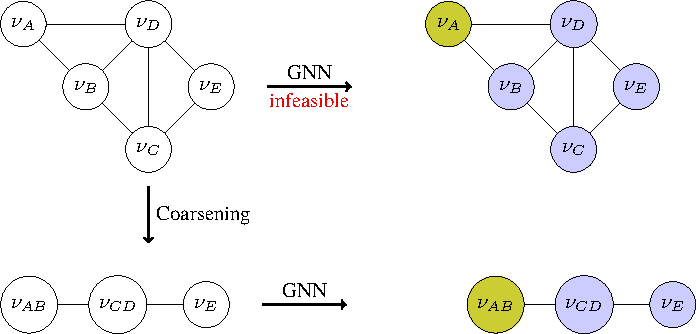
\includegraphics[width=\linewidth]{images/coarsening-illustration/coarsening-illustration.pdf}
		\end{tikzfigure}
	}

	\block{The performance-complexity trade-off}{
		\begin{tikzfigure}
			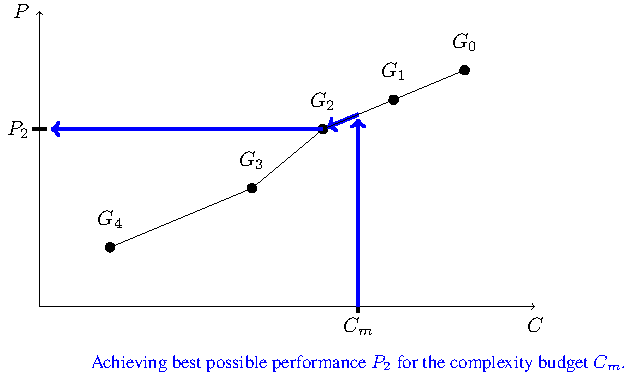
\includegraphics[width=\linewidth]{images/performance-complexity/performance-complexity.pdf}
		\end{tikzfigure}
	}

	\block{HARP pipeline overview}{
		\begin{tikzfigure}
			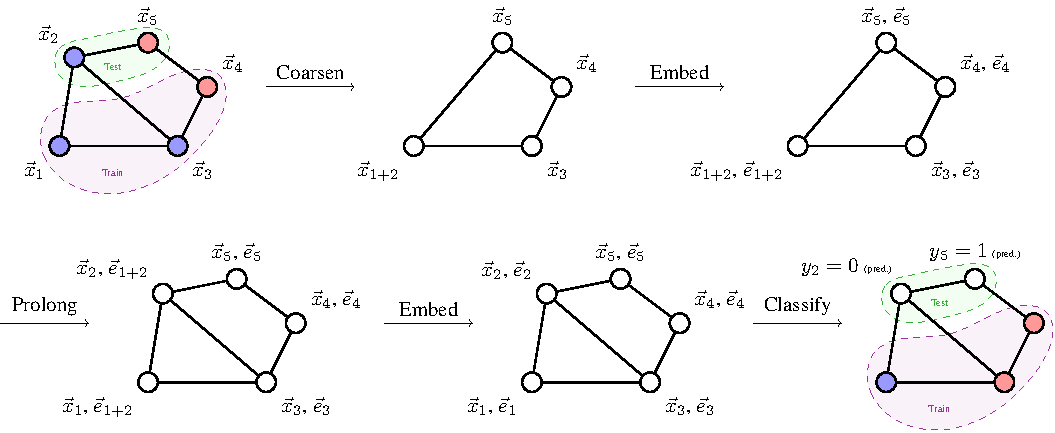
\includegraphics[width=\linewidth]{images/harp-overview/harp-overview.pdf}
		\end{tikzfigure}
	}

	\column{0.5}
	\block{Deep HARP}{
		\begin{tikzfigure}
			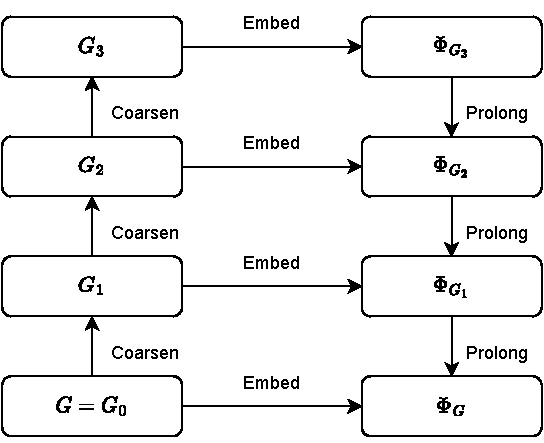
\includegraphics[width=0.5\linewidth]{images/deep-harp/deep-harp.pdf}
		\end{tikzfigure}
	}

	\block{Adaptive prolongation}{
		\begin{tikzfigure}
			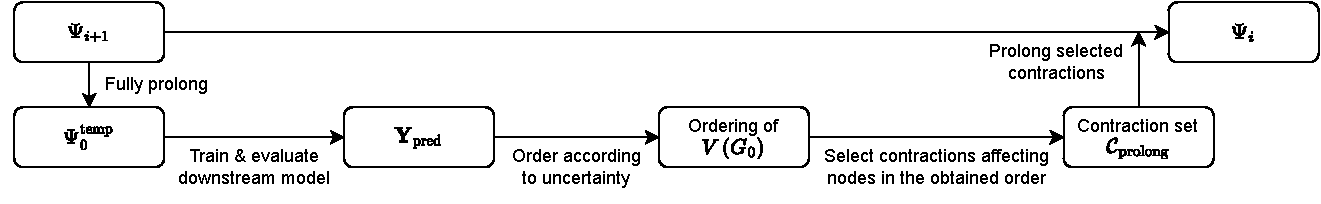
\includegraphics[width=\linewidth]{images/adaptive-prolongation/adaptive-prolongation.pdf}
		\end{tikzfigure}
	}

	\block{Results}{
		\begin{tikzfigure}
			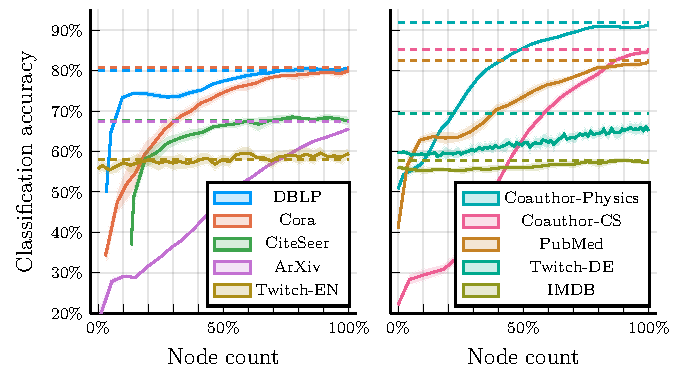
\includegraphics[width = \linewidth]{images/adaptive-coarsening/adaptive-coarsening.pdf}
		\end{tikzfigure}
		Downstream classifier accuracies at different steps of adaptive prolongation. Dashed line shows the baseline node2vec model accuracy. The node count is taken relative to the total node count in each dataset. The results are averaged over multiple runs, with the solid line representing the mean and the shaded area denoting one standard deviation.
	}
\end{columns}

\end{document}
